%%%%%%%%%%%%%%%%%%%%%%%%%%%%%%%%%%%%%%%%%%%%%%
\begin{figure}[h!]
     \centering
     \begin{subfigure}[b]{0.8\textwidth}
         \centering
         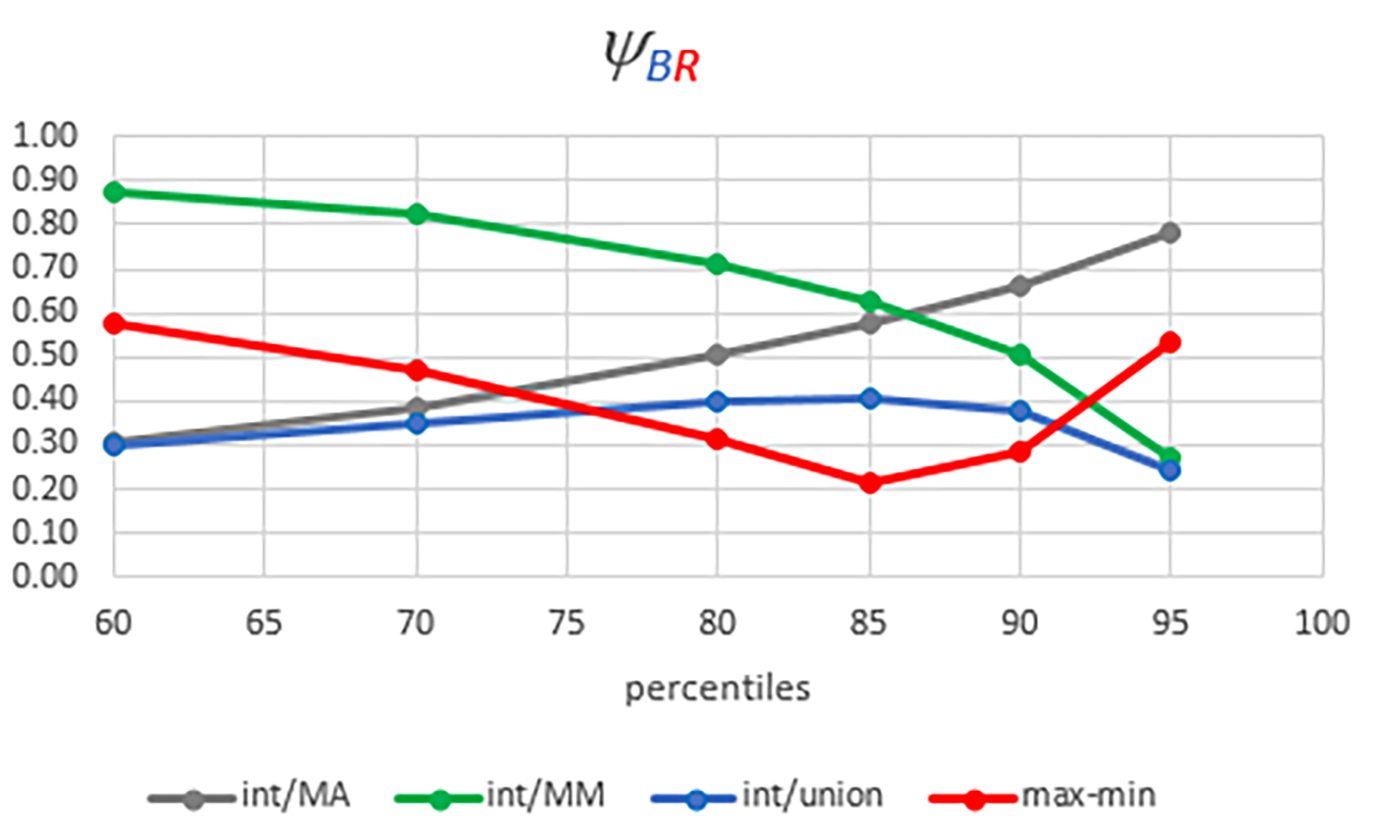
\includegraphics[width=\textwidth]{Imagenes/qibr.png}
         \caption{\textpsi \textsubscript{BR}}
         \label{psiBR}
     \end{subfigure}
     \hfill
     \begin{subfigure}[b]{0.8\textwidth}
         \centering
         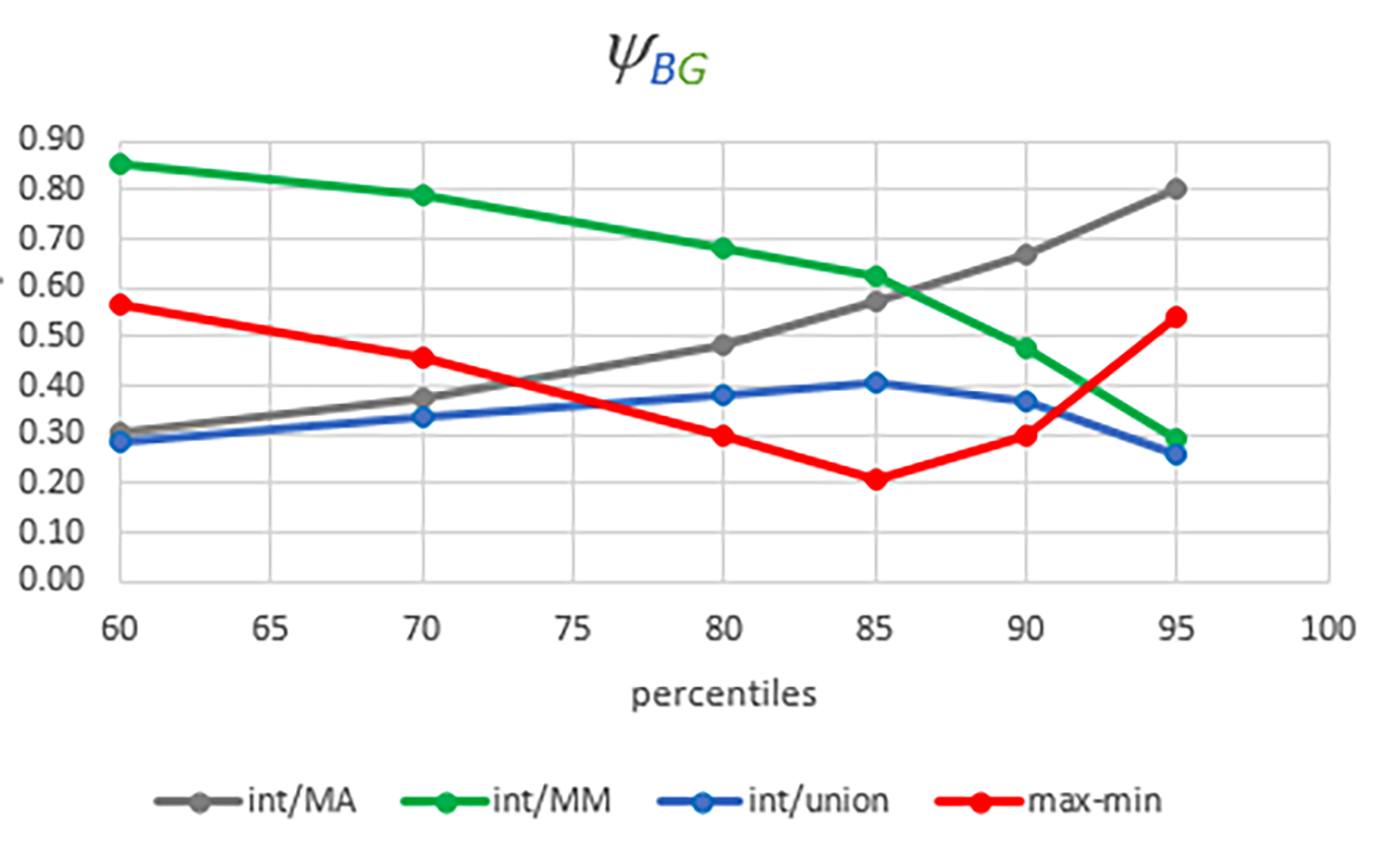
\includegraphics[width=\textwidth]{Imagenes/qibg.png}
         \caption{\textpsi \textsubscript{BG}}
         \label{psiBG}
     \end{subfigure}
     \hfill
     \begin{subfigure}[b]{0.8\textwidth}
         \centering
         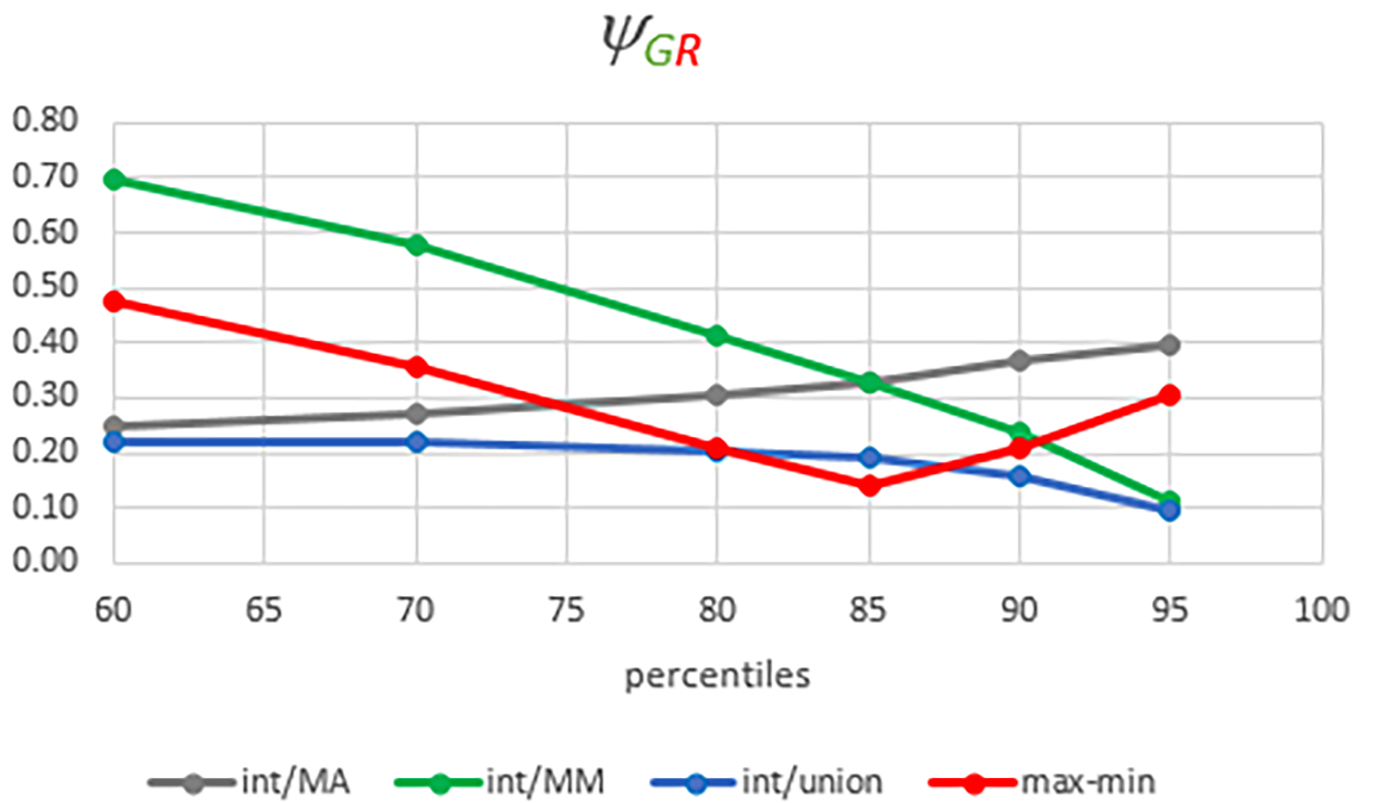
\includegraphics[width=\textwidth]{Imagenes/qigr.png}
         \caption{\textpsi \textsubscript{GR}}
         \label{psiGR}
     \end{subfigure}
        \caption{Índice de calidad}
        \label{quality_index}
\end{figure}

%tamaño
\begin{figure} [h!]
         \centering
         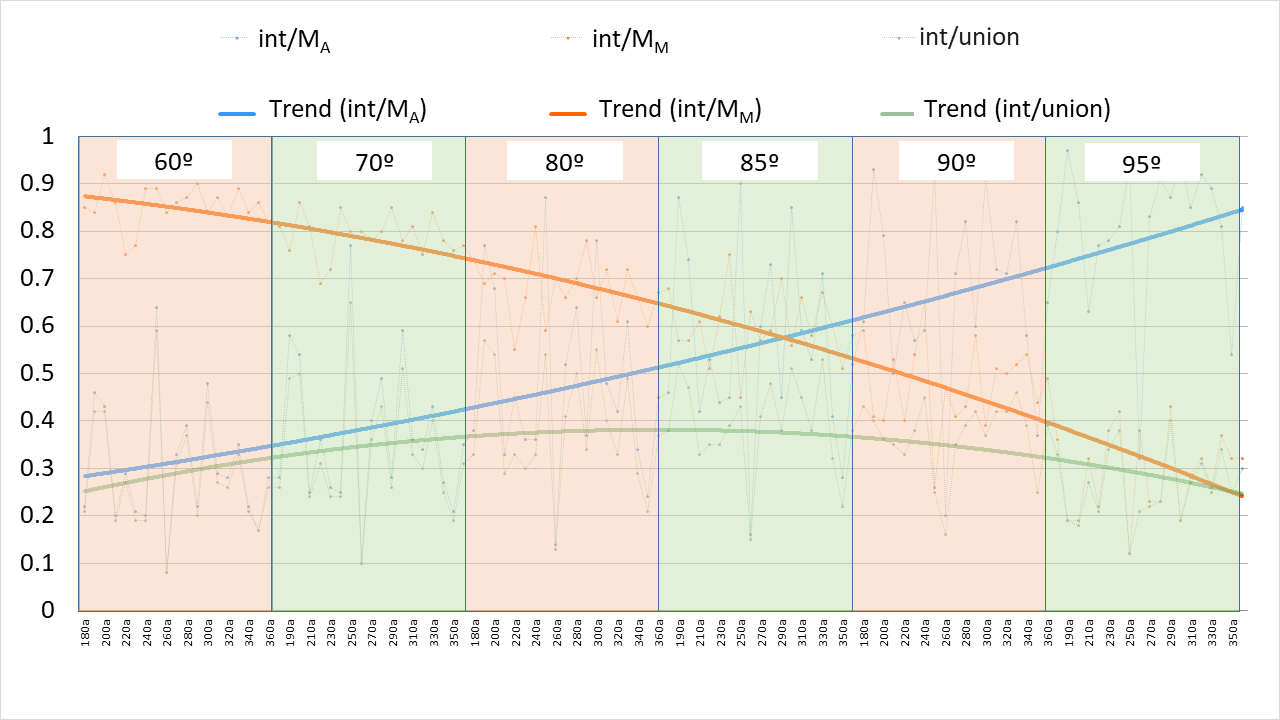
\includegraphics[width=\textwidth]{Imagenes/grafico.png}
         \hfill
         \caption{Dispersión y tendencia de los índices de calidad al variar el percentil del umbral (60º a 95º) usando el IIC resultado de la resta entre banda azul menos banda roja. Las líneas continuas representan la tendencia para cada índice, mientras que los puntos subyacentes corresponden a los valores obtenidos para cada imagen analizada.}
        \label{curvas_QI}
\end{figure}

%%%%%%%%%%%%%%%%%%%%%%%%%%%%%%%%%%%%%%%%%%%%%%
